\newpage
\subsection{Fase 2: Selección de datos}
En esta etapa se obtuvo el un conjunto de datos de \textit{Morbilidad por cáncer en Pereira} entre los años 2019 y 2021. Cabe resaltar, que los datos fueron solicitados a la secretaria de salud de la alcaldía Municipal de Pereira por medio de la pagina \textit{https://www.datos.gov.co/}. Este conjunto de datos consta de un tamaño de $40.658$ filas y $7$ columnas: 
\begin{itemize}[label=\SquareShadowTopLeft]
	\item  \textit{\textbf{NOMBRE DIAGNOSTICO:}} 	
	Nombre de la enfermedad.
	\item  \textit{\textbf{CÓDIGO DIAGNOSTICO:}} 	
	Códigos únicos de procedimientos en salud, código que identifica el diagnostico.
	\item  \textit{\textbf{EDAD:}} 	
	Edad del paciente.
	\item  \textit{\textbf{SEXO:}} 	
	Sexo del paciente.
	\item  \textit{\textbf{ZONA:}} 	
	Zona rural o urbana donde vive el paciente.
	\item  \textit{\textbf{RÉGIMEN:}} 	
	Tipo de vinculación de la persona al sistema general de salud .
	\item  \textit{\textbf{AÑO:}} 	
	Año en que se realiza el diagnostico.
\end{itemize}

A continuación, se realizó un \textit{Análisis exploratorio de datos} para descubrir patrones generales en el conjunto de datos propuesto. En primer lugar, se determino que el código $C509$, relacionado a un tumor maligno de la mama con una localización no especificada, es el mas tipo de cáncer mas frecuente de la totalidad del conjunto de datos, para lograrlo se utilizó la representación gráfica de nube de palabras que se muestra en la figura \ref{WORD_CLOUD}.

\begin{figure}[h!]
	\centering
	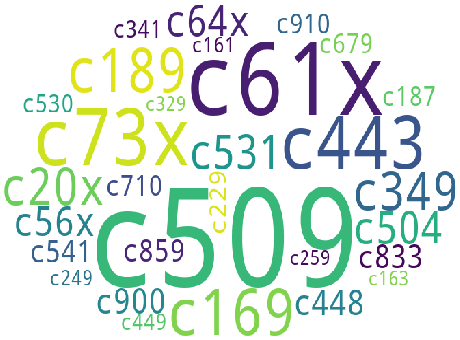
\includegraphics[width=0.84
	\linewidth]{IMAGENES/WORD_CLOUD}
	\caption{Nube de palabras con los tipos de cáncer frecuentes.}
	\label{WORD_CLOUD}
\end{figure}

Dadas las variables anteriores, se seleccionaron aquellos registros de los pacientes que fallecieron por tumores producidos por cáncer de mama según el manual de codificación y estadificación del programa de Vigilancia, Epidemiología y Resultados Finales \textit{SEER} \footnote{SEER: Surveillance, Epidemiology, and End Results}. Cabe resaltar, que este programa brinda información sobre las estadísticas del cáncer en un esfuerzo por reducir la morbilidad causada por esta enfermedad en Estados Unidos \cite{SEER2022}. El filtrado de los registros fue realizado a través de la variable \textit{CÓDIGO DIAGNOSTICO} según los códigos topográficos del $C500$ al $C509$ especificados por la SEER para la clasificación de Tumores múltiples causados por cáncer de mama clasificados tal y como se describe en la tabla \ref{Tabla_SEER}. 

\begin{table}
	\begin{threeparttable}[hbt!]
		\caption{Directrices de codificación Seno C500 - C509.}
		\label{Tabla_SEER}
		\begin{tabular}{ p{2cm} p{6cm}} \toprule
			Código 
			&Localización           
			\\ \hline	
			%-------------------------------------------
			C500
			& \begin{enumerate}
				\item Pezón (aerolar)
				\item Enfermedad de Paget sin tumor subyacente
				\item Despliegue 
			\end{enumerate}
		
			\\ \hline
			C501
			& \begin{enumerate}
				\item Porción central de la mama (sub-aerolar) que se extiende 1 cm alrededor del complejo areolar
				\item Retro-aerolar
				\item Infra-aerolar
				\item Junto a la areola, NOS
				\item Detrás, debajo, debajo de, al lado de, encima de, cefálico a, o debajo del pezón
				\item Enfermedad de Paget con tumor subyacente
				\item Central inferior
			  \end{enumerate}
		
			\\ \hline
			C502
			& \begin{enumerate}
				\item Cuadrante superior interno (UIQ) de la mama
				\item Medial superior
				\item interior superior
			\end{enumerate}
			
			\\ \hline
		   C503
			& \begin{enumerate}
				\item Cuadrante inferior interno (CI) de la mama
				\item Medial inferior
				\item Medial bajo
				\item Inferior interno
			\end{enumerate}
		
			\\ \hline
			C504
			& \begin{enumerate}
				\item Cuadrante superior externo (UOQ) de la mama
				\item Lateral superior
				\item Superior externo
				\item Lateral alto
			\end{enumerate}
		
			\\ \hline
			C505
			& \begin{enumerate}
				\item Cuadrante inferior externo (LOQ) de la mama
				\item Lateral inferior
				\item Inferior externo
				\item Lateral bajo
			\end{enumerate}
		
			\\ \hline
			C506
			& \begin{enumerate}
				\item Cola axilar de la mama
				\item Cola de la mama, NOS
				\item Cola de Spence
			\end{enumerate}
		
			\\ \hline
			C508
			& \begin{enumerate}
				\item Lesión superpuesta de la mama
				\item Mama inferior, NOS
				\item Mama interior, NOS
				\item Mama lateral, NOS
				\item Mama baja, NOS
				\item Mama medial, NOS
				\item Pecho medio, NOS
				\item Mama externa, NOS
				\item Mama superior, NOS
				\item Seno superior, NOS
				\item 3:00, 6:00, 9:00, 12:00 horas
			\end{enumerate}
		
		  \\ \hline
			C509
			& \begin{enumerate}
				\item Pecho, NOS
				\item Toda la mama
				\item Múltiples tumores en diferentes sub-sitios dentro de la mama
				\item Inflamación sin masa palpable
				\item 3/4 o más de la mama afectada por el tumor
				\item Difuso (tamaño del tumor 998)
			\end{enumerate}
		   %-------------------------------------------
		   
		\\ \hline	
		\end{tabular}
	\end{threeparttable}
\end{table}

\newpage
De manera similar, la SEER determina que la posición del tumor en la mama puede describirse por medio las posiciones del reloj tal y como se muestra en la figura \ref{Breast_Clock}.

\begin{figure}[h!]
	\centering
	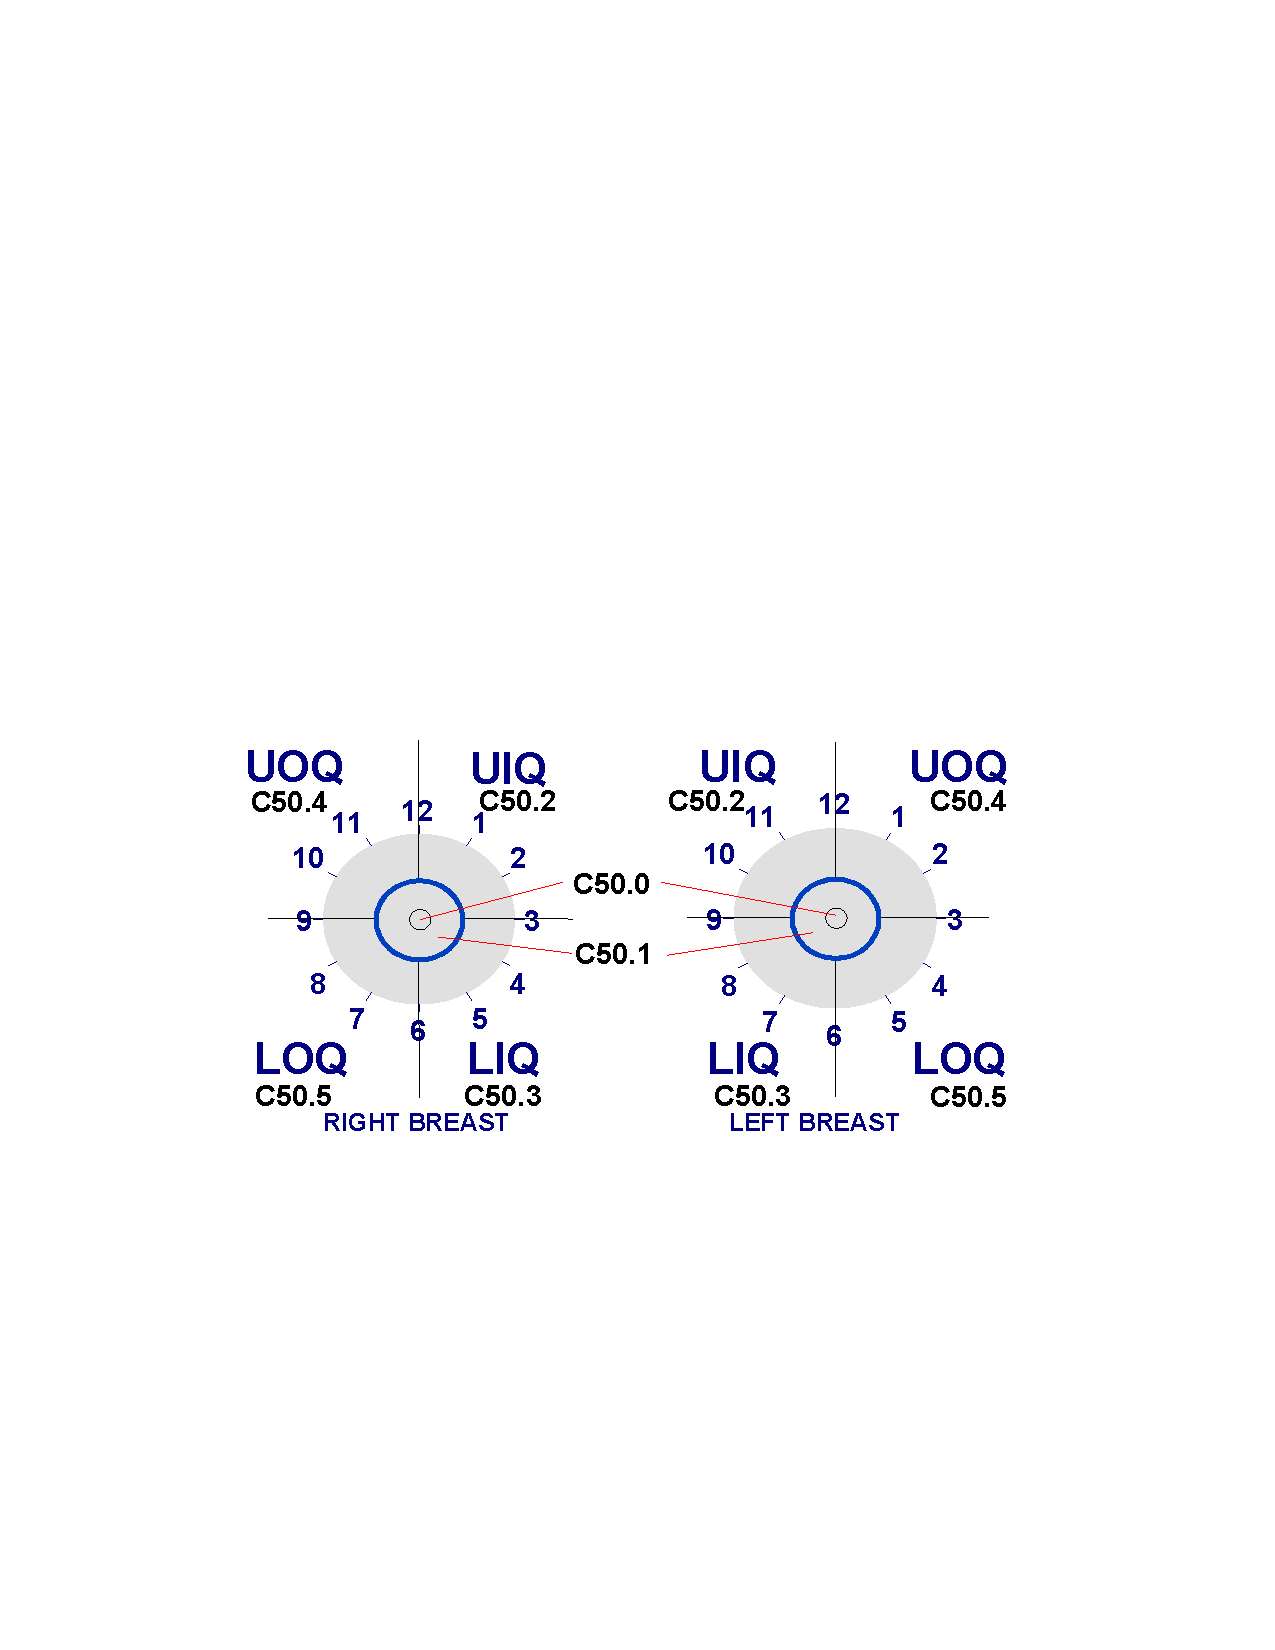
\includegraphics[width=1
	\linewidth]{IMAGENES/BREAST_CLOCK_POSITION}
	\caption{Posiciones del reloj y códigos de los cuadrantes de los senos.}
	\label{Breast_Clock}
\end{figure}

En consecuencia, de  realizar el filtrado del conjunto total de datos se obtuvo un conjunto de datos resultante de $8927$ registros. Teniendo en cuenta en nuevo conjunto de datos se generaron las gráficas que puede observarse en la figura \ref{EDA}. Dados los resultados obtenidos, se determina que  el código de diagnostico de cáncer de mama con mas numero de muertes asociadas fue el $C509$, seguido por el $C504$ respectivamente. 

\begin{figure}[h!]
	\centering
	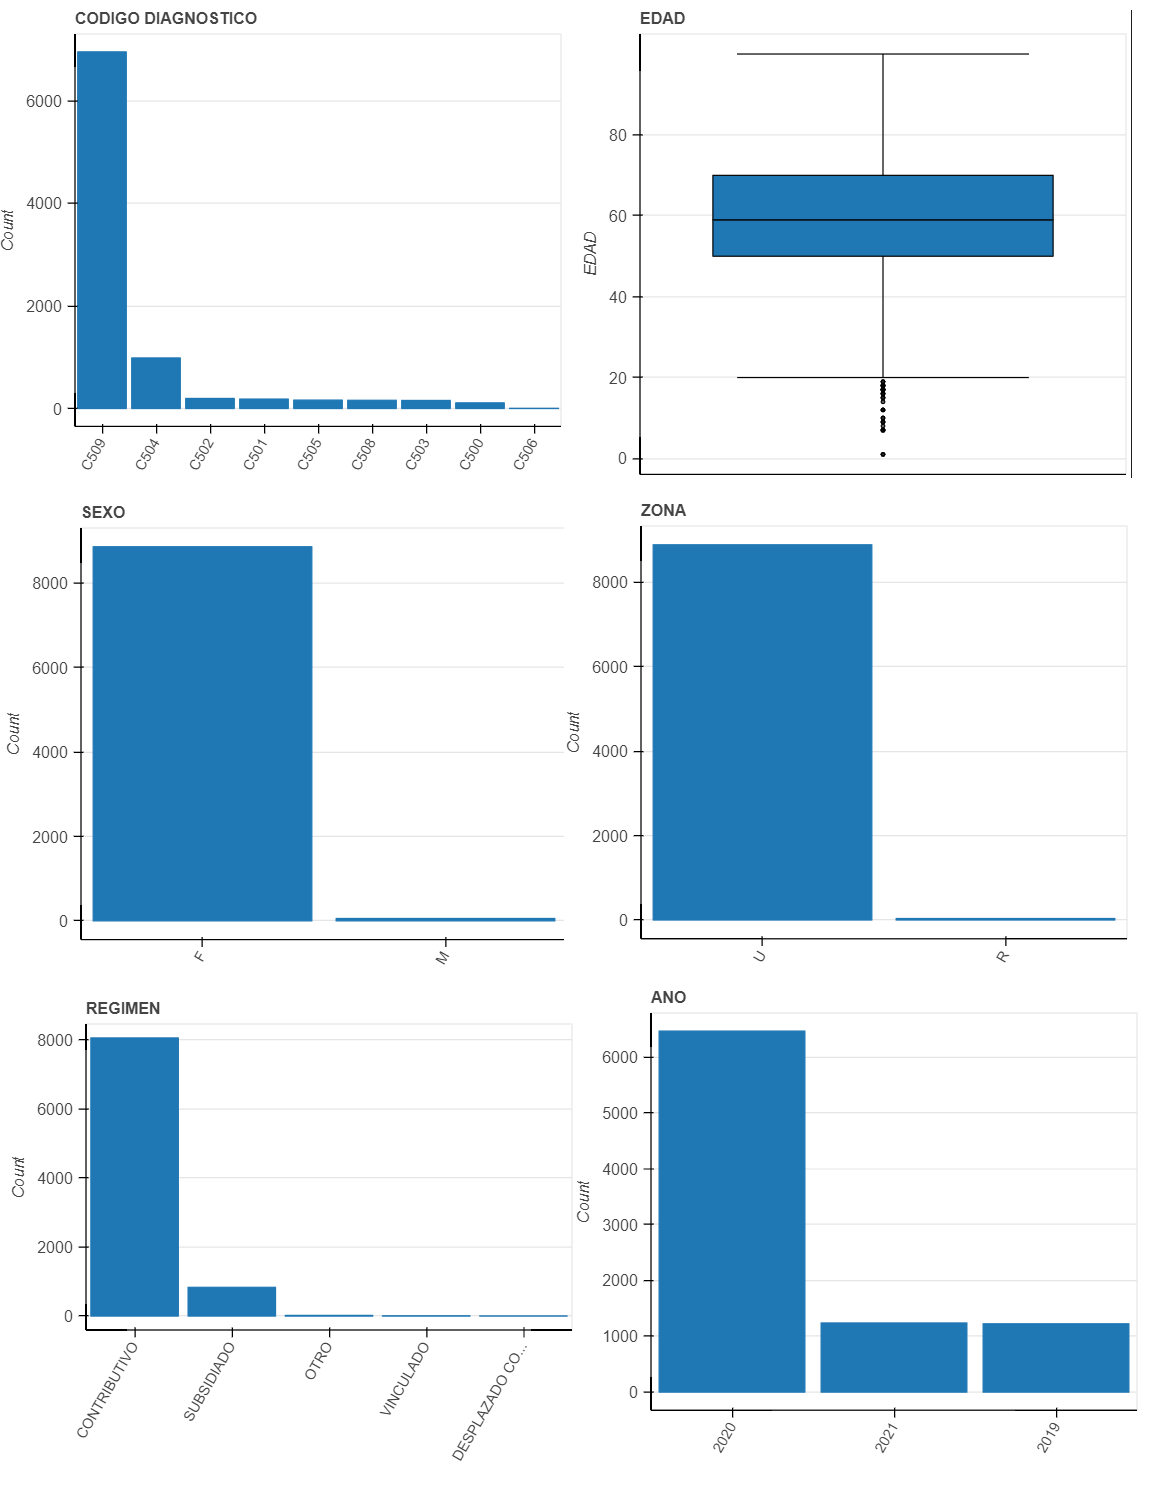
\includegraphics[width=1 
	\linewidth]{IMAGENES/EDA_BREAST}
	\caption{Diagramas analíticos cáncer de Seno C500 - C509.}
	\label{EDA}
\end{figure}

\newpage 
De igual modo, es plausible afirmar que el conjunto de datos presenta 5 variables de tipo \textit{categórica} y 2 de tipo \textit{numérica}. Adicionalmente, según los resultados obtenidos en la figura \ref{EDA}, se determina que el genero femenino entre los 50 y 70 años de edad, que habitan en zonas urbanas y que tienen una vinculación de salud de régimen contributivo presentan un mayor numero de morbilidad por cáncer de mama. Por otro lado se infiere, que en el año 2020 se presento una tasa mayor de muertes con respecto a los años 2018 y 2021.

